% !TEX root = ../thesis.tex
\chapter{Lit Review}
	\label{chap:lit_review}
	Education and the sharing of knowledge is a powerful tool. In fact, in our opinion the most important skill anyone can have. As a famous quote said, "give a man a fish, and he will starve, but teach him to fish, and he won't be hungry anymore". However, it wasn't until 1918 that education, as most people in England and Wales have experienced, started to come into effect \cite{education1918}.
	
	Education over the years was very much about just giving the knowledge to the students from the teacher. It wasn't until 1988, under the Education Reforms Act 1988, that assessments got introduced. The introduction was through the introduction of the national curriculum in England and Wales \cite{education1988}.
	
	As the curriculum got rolled out, statutory assessments got introduced to education between 1991 and 1995. Key Stage 1 first, followed by Key Stages 2 and 3, respectively.[1] Only for the core subjects of English, Mathematics and Science had the assessments first introduced. The first assessments in Key Stage 1 were a range of cross-curricular tasks to be delivered in the classroom, known as standardised assessment tasks - hence the common acronym 'SATs'. However, the complexity of the use of these meant more formal tasks quickly replaced them.[1] The assessments in Key Stages 2 and 3 were developed using more traditional tests.
	
	In all 3 Key Stages, tests became the main form of statutory assessment, but a separate strand of Teacher Assessment was also used. This allowed teachers to make judgements about pupils they taught, based on their knowledge of the pupil's learning and attainment against the attainment targets contained within the national curriculum. The results of both tests and teacher assessments were reported using a common scale of attainment levels, numbered 1 to 8 across the three key stages, with the national expectation that pupils would achieve Level 2 at the age of 7; Level 4 at the age of 11; and Level 5 or 6 by the age of 14.
	
	This model continued, with minor adjustments to reflect the changing content of the National Curriculum, up to 2004. From 2005, the role of the tests was downplayed at Key Stage 1, with tests being used only internally to support teacher assessment judgements.[2] Further changes came in 2008 when the government announced that testing in Key Stage 3 was to be scrapped altogether.[3]
	
	In 2013, then Education Minister, Michael Gove announced that when the new version of the National Curriculum was introduced to schools from 2014, the system of attainment levels would be removed.[4] As a result, since 2016, the old system has levels that are no longer used as part of statutory assessment. Instead, tests and teacher assessments now follow different models at each key stage.
	
	\section{The Purpose of Assessment, Marking and Feedback in Education}
	
	
	\section{Traditional Methods of Marking and Providing Feedback} % Should these be subsections?
	
	
	\section{Why Traditional Traditional Marking and Feedback Methods are Effective}
	
	
	\section{The Negative Aspects of Traditional Marking and Feedback Methods}
	
	
	\section{What is Comparative Judgement} 
		Comparative judgement is a mathematical way to determine which observation item is better than the other item also being observed compared to each other. This method was first proposed in 1927 by Louis Leon Thurstone, a psychologist, under the term "the law of comparative judgement" \cite{thurstone1927psychophysical, thurstone1927law}. In modern-day terminology, it gets more aptly described as a model used to obtain measurements from any pairwise comparison process. Examples of such methods are comparing the perceived intensity of physical stimuli, such as the weights of objects, and comparing the extremity of an attitude expressed within statements, such as statements about capital punishment. The measurements represent how we perceive things rather than being measurements of actual physical properties. This kind of measurement is the focus of psychometrics and psychophysics. <wikipedia>
		
		In more technical terms, the law of comparative judgment is a mathematical representation of a discriminal process. This process involves a comparison between pairs of a collection of entities concerning multiple magnitudes of attributes. The model's theoretical basis is closely related to item response theory and the theory underlying the Rasch model. These methods are used in psychology and education to analyse data from questionnaires and tests.
		<wikipedia>
		
		While comparative judgement is a technique that has been around for almost 100 years, it wasn't until the early nineties that this technique got proposed for use within an educational setting. This first proposal was by Politt and Murry \cite{pollitt1996raters}, who conducted a study where they tested candidates on their English proficiency within Cambridge's CPE speaking exam. The judges watched 2-minute videos and judged which one out of a pair of videos they deemed better at the requested task in the exam. However, before this, in the ninety seventies and eighties, comparative judgement was presented as a more theoretical basis for educational assessments \cite{andrich1978rating}. 
		
		With the momentum of his findings, Politt then presented comparative judgement as a tool for exam boards to use to be able to compare the standards of A-Levels from the different exam boards, replacing the direct judgement of a script that was at the time currently being used \cite{newton2007paired}. In his papers titled, "Let's Stop Marking Exams" \cite{stop_marking_pollitt}, he presents a valid argument for using comparative judgement, with the advantages it brings over some traditional types of marking.
		
		Politt, in 2010, also presented a paper at the Association for Educational Assessment – Europe. It was about How to Assess Writing Reliably and Validly. Politt presented evidence of the extraordinarily high reliability achieved with Comparative Judgement in assessing primary school pupils' skill in first-language English writing \cite{pollitt2009abolishing}.
		
	\section{The Logic Behind Comparative Judgement and What it Aims to Do} % Should these be subsections?
		How comparative judgement works is to present two options to a marker. The marker then gets asked to pick which one of the two options they think is the better one. The marker will get presented with all possible combinations available, each time picking which one they think is the better one out of the two. An outputted score is then presented based on the method used. The original method, the Law of Comparative Judgement (LCJ), follows the formula:
		
		\begin{figure}[h]
			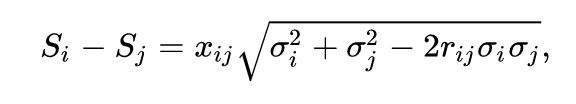
\includegraphics[width=8cm]{graphics/LCJ_formula.png}
			\caption{}
			\centering
		\end{figure}
	
		 $S_{i}$ is the psychological scale value of stimuli $i$
		%{\displaystyle x_{ij}} is the sigma corresponding with the proportion of occasions on which the magnitude of stimulus i is judged to exceed the magnitude of stimulus j
		%{\displaystyle \sigma _{i}} is the discriminal dispersion of a stimulus {\displaystyle R_{i}}
		%{\displaystyle r_{ij}} is the correlation between the discriminal deviations of stimuli i and j
		%The discriminal dispersion of a stimulus i is the dispersion of fluctuations of the discriminal process for a uniform repeated stimulus, denoted {\displaystyle R_{i}}, where {\displaystyle S_{i}} represents the mode of such values. Thurstone (1959, p. 20) used the term discriminal process to refer to the "psychological values of psychophysics"; that is, the values on a psychological continuum associated with a given stimulus.
		
		However, an alternative version derived from Louis Leon Thurstone, referred to as the "Pairwise Comparison" \cite{thurstone1927law}, will provide an output based on the difference between the quality values is equal to the log of the odds in respect to object-A will be object-B. This formula gets represented as: 
		$\displaystyle \mathrm {log\;odds} (A\ {\text{beats}}\ B\mid v_{a},v_{b})=v_{a}-v_{b} $.
		
		$\Pr\{X_{ji}=1\}={\frac {e^{{\delta _{j}}-{\delta _{i}}}}{1+e^{{\delta _{j}}-{\delta _{i}}}}}=\sigma (\delta _{j}-\delta _{i})$
		
		 .
		%\displaystyle \mathrm {log\;odds} (A\ {\text{beats}}\ B\mid v_{a},v_{b})=v_{a}-v_{b}}		


	\section{How effective is Comparative Judgement at Providing Feedback?} % Should these be subsections?
		
		

	\section{Related Work}
		\label{sec:google_fu}



	\subsection{Subsection all similar work}
		\label{sec:resources_bibtex}
	


	\subsection{Comparison of similar work}
